\section{Applications of Causality}
\label{sec:application}
% siyuan: 这里需要写一下,把causality用在这些任务上的motivation是 这些任务具有时序性,通过causality可以补全不完整的症状序列(post中不一定完全体现这个人的症状)

% Causal relationships inferred from social media data can be validated not only through existing literature (to be discussed in Section \ref{sec:exp}) but also applied to improve performance in various downstream tasks. \MY{Remarkably, a number of causal relationships discerned from social media posts correspond with established clinical findings xxxx. More significantly, this paper further delves into how these causal features can be effectively utilized for disease detection.}

In this section, we show that we can discover reliable causal relationships that can also be supported with established clinical findings (Section \ref{sec:analysis}), and how these causal features can be effectively utilized for mental disorder detection (Section \ref{sec:causal_as_feature}).

% Remarkably, a number of causal relationships discovered from social media posts correspond with established clinical findings (to be discussed in Section \ref{sec:analysis}). 
% Moreover, we further delve into how these causal features can be effectively utilized for mental disorder detection (Section \ref{sec:causal_as_feature}).

\begin{table*}[th]
\resizebox{\textwidth}{!}{

    \small
    \centering
    \begin{tabular}{l|l|c|c|c}
    \hline
    Cause Symptom & Result Symptom & Supported/Disagreed & ATE & References  \\ 
    \hline
     fears of being negatively evaluated  & poor memory & Disagreed & 0.894 &  \citet{seinsche2023memory}\\ 
     fears of being negatively evaluated  & Depressed Mood & Supported & 0.886 & \makecell[c]{\citet{jacobson2017anxiety} \\ \citet{kim2019cultural}} 	 \\ 
    fears of being negatively evaluated & Suicidal ideas & Supported & 0.874 & \citet{klumpp2023objective} \\
    Hyperactivity agitation & Impulsivity & Disagreed & 0.869 &  \citet{grandjean2021stronger} \\ 
    fears of being negatively evaluated & \makecell[l]{do things easily get painful \\consequences} & Supported & 0.857 & \makecell[c]{\citet{moscovitch2018autobiographical} \\ \citet{Chu2016ThwartedBM}} \\ 
    panic fear & somatic symptoms sensory & Mixed & 0.855 & \makecell[c]{\citet{ehlers1993interoception} \\\citet{kang2024pontomesencephalic}} \\ 
    fears of being negatively evaluated & Autonomic symptoms & Supported & 0.855 & \makecell[c]{\citet{alvares2013reduced} \\\citet{weeks2016fears}} \\ 
    panic fear & \makecell[l]{Decreased energy tiredness \\fatigue} & Supported & 0.845 & \citet{pasquini2015fatigue} \\
    \hline
    \end{tabular}}
    \caption{Systematic literature review of the top eight causal relationships with the highest ATE scores.}
    \label{tab:error_analysis}

\end{table*}

\subsection{Inferred Causal Relationships} % this part is not finished yet
\label{sec:analysis}

We can automatically discover various causal relationships from social media with the method mentioned above. To validate their reliability, we also conduct literature reviews, and find that many of them can be supported by existing studies. 

We show some examples in Table \ref{tab:causal_analysis}. We can see that some of the conclusions are intuitive, like breakdown will increase the risk of future depression. However, others are more subtle, such as irritability can cause weight change. We then find that, according to \citet{vanzhula2019illness}, the relationship between eating and irritability stands out a crucial pathway influencing comorbidity between Post-Traumatic Stress Disorder (PTSD) and Eating Disorders (EDs). 

To highlight discrepancies between our findings and existing literature, we further examine the top eight causal relationships with the highest ATE scores in Table \ref{tab:error_analysis}.
Among these, five relationships are supported by existing literature. Two relationships show disagreement to some extent, proposing alternative associations. An example is \citet{seinsche2023memory}'s finding suggesting a connection between social anxiety and a clearer memory about distasteful social situations, which is contradict to our causal link between fear of being negatively evaluated and poor memory. Moreover, one finding got mixed results, depending on studies and samples.
Overall, existing literature mostly focuses on symptom-disease causality, providing limited evidence to direct causal examinations between pairs of symptoms. Our current findings have the promise of inspiring future studies focusing on direct causal relationship examinations on pairs of symptoms.


\begin{figure}[h]
	\centering
	\includegraphics[width=\linewidth]{figures/ate_syp_365.pdf}
	\caption{Visualization results for the causality between life events and symptoms with the time window of 1 year. The size of LEs nodes reflects the number of related symptoms, and the thickness of the lines indicates the strength of the causal relationship (ATE).}
	\label{fig:LEs_symps_disease}
\end{figure}


To make the intricate relationships more intuitive, Figure \ref{fig:LEs_symps_disease} illustrates a visual representation of the causal relationships between life events (LEs) and symptoms, shedding light on the intricate connections within the context of anxiety. Note that previous works predominantly focus on establishing connections between diseases and life events, while the association between symptoms and LEs is less explored in existing literature. Therefore, our examination of these relationships can provide valuable insights into the intricate web of factors contributing to mental health outcomes.

Moreover, our method can not only find casual relationships qualitatively, but also measure their effects quantitatively with ATE. This enables us to incorporate these findings as numerical features for mental disorder detection algorithms. 

% Prev Version
% Using the mentioned method, we obtained two types of causality. To illustrate the practical implications of the causal relationships obtained in our experiments, we present some specific instances supported by relevant literature in Table \ref{tab:causal_analysis}.

% According to \citet{vanzhula2019illness}, the relationship between eating and irritability stands out a crucial pathway influencing comorbidity between Post-Traumatic Stress Disorder (PTSD) and Eating Disorders (EDs). The study suggests that symptoms of PTSD may contribute to the maintenance of EDs through triggers such as disturbing dreams, leading to a preoccupation with weight or shape.

% Moreover, \citet{boschloo2015network} observed that symptoms from different diagnostic categories, which do not necessarily overlap, can exhibit strong connections. For instance, the study found a strong connection between low mood (associated with a major depressive episode) and hyperactivity disorder.
% Further, \citet{konac2021comorbidity} mentioned that peer relationship problems are one of the most prominent risk factors, acting as a bridging node connecting certain symptoms of depression and generalized anxiety disorder worries.

% It is noteworthy that while the association between symptoms and LEs is less explored in existing literature, the focus has predominantly been on establishing connections between diseases and life events. This observation emphasizes the novel contribution of our study in examining the relationships between symptoms and life events, providing valuable insights into the intricate web of factors contributing to mental health outcomes.

% \citet{vanzhula2019illness} studied illness pathways between eating disorder(ED) and PTSD symptoms.They mentioned that eating–irritability may be a crucial illness pathway by which comorbidity is maintained between PTSD and EDs.Moreover, PTSD symptoms might maintain EDs via reminders of trauma (e.g., disturbing dreams), triggering self-critical thoughts about one's body, and preoccupation with weight or shape.This aligns with the first and second rows in table \ref{tab:causal_analysis}.
% Using the mentioned method, we obtained the two types of causality. The significance of causality is measured by the magnitude of the Average Treatment Effect (ATE) values\MY{We have defined it previously, no need to use full name again. But this argument needs citation}. Here, ATE values indicate how much the probability of other symptoms increases when a symptom/life event occurs.

% Here, we present the causality between symptoms for time windows of 30 days(Table \ref{tab:syp_causal_30}), 90 days(Table \ref{tab:syp_causal_90}), and 180 days(Table \ref{tab:syp_causal_180}), along with the causality between life events and symptoms. Specifically, for the causality between life events and symptoms, we only showcase the results for a time window of 1 year(Table \ref{tab:LEs_causal_365}). For each time window, we display the top 5 results based on the magnitude of the Average Treatment Effect (ATE) values.

% \MY{You can add a subsection here to illustrate what we get from the previously mentioned approach, move part of Section 6's analysis here, this is like the product you obtain. Here you can mention different window sizes and give them names, i.e. symp-symp causal {window = xx xx}... It will make your experimental results part easier to understand. In Sec 6, you should focus on case analysis, that what kind of causal relation contributes to your final improvement on DPD and ERD.}


% To make the intricate relationships more intuitive, Figure \ref{fig:LEs_symps_disease} illustrates a visual representation of the causal relationships between life events (LEs) and symptoms, shedding light on the intricate connections within the context of anxiety. Originating from LEs, lines establish connections to associated symptoms, with the thickness of the lines indicating the strength of causality. Finally, the symptoms are aggregated according to diseases.

% Notably, the nodes in the graph serve distinct roles: green nodes represent life events (LEs). Blue nodes represent somatic symptoms. Yellow nodes represent psychological symptoms. Red nodes represent diseases-specifically, in this instance, anxiety. The size of the LEs nodes reflects the potential impact, measured by the number of symptoms they may induce. The thickness of the lines connecting LEs nodes to symptom nodes represents the magnitude of the Average Treatment Effect (ATE) values, indicating the strength of the causal relationship.



\subsection{Causality as Feature}
\label{sec:causal_as_feature}
Given the chronological nature of causal relationships, we leverage them in two temporal tasks: Diagnosis Point Detection and Early Risk Detection, both of which involve the detection of mental disorders along a continuum. The two tasks are illustrated in Figure \ref{fig:tasks}, and we briefly introduce them here:
 % \KZ{There is no such thing as ``diagnosis point''. I myself don't know what's the right phase for it. Please check.}
\begin{figure}[th]
	\centering
	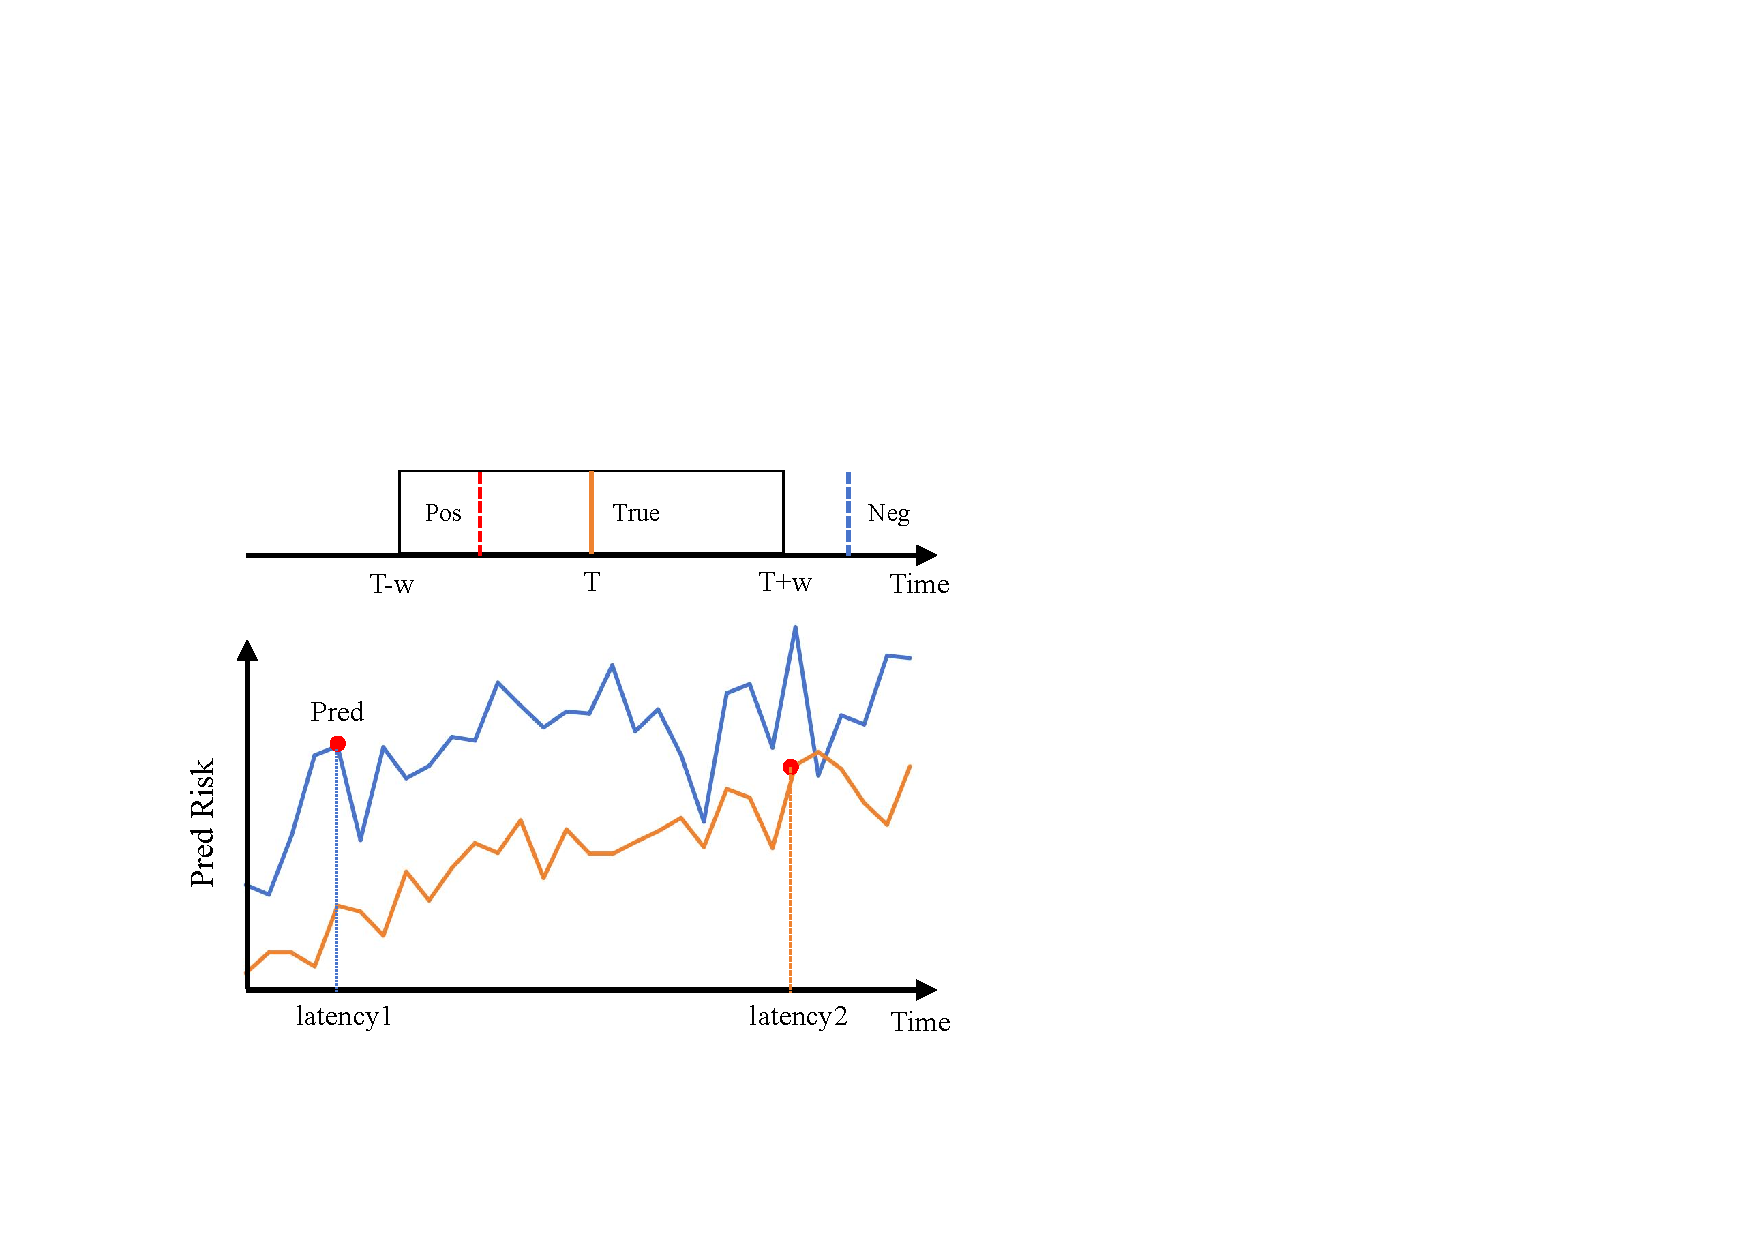
\includegraphics[width=0.9\linewidth]{figures/task_fig.pdf}
	\caption{Illustration of the DPD and ERD task. For DPD, we want the predicted time to fall in a window $w$ of the actual diagnosis point $T$. Prediction with in $[T-w, T+w]$ will be considered positive, otherwise negative. For ERD, we want to predict the risk of a patient as soon as possible (the lower latency, the better), while not making false alert for non-patients.}
	\label{fig:tasks}
\end{figure}

\paragraph{Task 1. Diagnosis Point Detection (DPD)} refers to the identification of the specific time window when a mental disorder is diagnosed in an individual according to their social medial posts. This temporal insight into the diagnosis is valuable because one’s mental health state is not static. 
For this task, \citet{macavaney-etal-2018-rsdd} proposed a dataset named RSDD-Time, which includes 598 manually annotated self-reported depression diagnosis Reddit posts that include temporal information about the diagnosis. The complete posting history can be found in the original RSDD dataset~\cite{yates-etal-2017-depression}.

\paragraph{Task 2. Early Risk Detection (ERD)} aims to detect mentor disorders in early stage~\cite{losada2016test,zhang2022psychiatric}. It can enable early interventions to half the effort and double the results. Here we focus on the ERD of Depression.

In the ERD setting, for a user $U_i$ with posts $[P_{i,1}, P_{i,2}, ..., P_{i,n}]$ in their posting history (where $n$ is the total number of posts, and $P_{i,j}$ is the $j$-th user-generated post of $U_i$), posts come one by one. Therefore, only $[P_{i,1}, P_{i,2}, ..., P_{i,t}]$ is available to the model at the $t$-th time. The model can make an early prediction of $y_i$ at $t (t \leq n)$ once it is confident enough, such that the prediction can make a good tradeoff between accuracy and earliness. 

The ERD task doesn't require additional temporal annotations in the dataset, as we care about earliness rather than the exact diagnosis point. Thus, experiments can be conducted using any self-reported depression diagnosis dataset, such as RSDD.

\paragraph{Method of applying causality}

To incorporate causal relationships into these two tasks, our primary motivation can be summarized as ``constructing a more comprehensive daily symptom sequence''. For user $U$, their daily symptom sequence can be denoted as $[S_{1}, S_{2}, ..., S_{n_d}]$, where $n_d$ is the total number of days during the posting history, and $S_{i}$ means the symptom vectors inferred from the $i$-th day's user-generated posts of $U$.

% \KZ{You need to define what is a symptom sequence, for the first time. Is it a sequence of symptom vectors of dimension 38? And there is one vector per day, or one vector per post. I also think the key here is not a more comprehensive symptom sequence, but rather a ``complete'' daily symptom sequence. Please be very specific about it. You want to infer the symptom vectors for those days that the user didn't post.}

As Figure \ref{fig:causal_apply} shows, social media posts may not capture the entirety of an individual's symptom evolution, as users may not share their experiences at all times when symptoms occur. Therefore, the symptom sequence identified from a single post will be incomplete. However, the extracted causal relationships can serve as a universal feature to bridge the gaps in these incomplete symptom sequences. As the example shown in Figure \ref{fig:causal_apply}, when we have obtained several ``life-event-to-symptom'' causal relationships (e.g., ``Relationship Conflicts and Breakdown'' causing "Indecisiveness" with an ATE value of 0.593), we can infer that the user is likely to experience the symptom of ``Indecisiveness'' even when the user posts nothing.
Now we can formalize the method of applying these causal relationships, taking ``symptom-to-symptom'' relationships as an example.  
\begin{figure}[th]
	\centering
	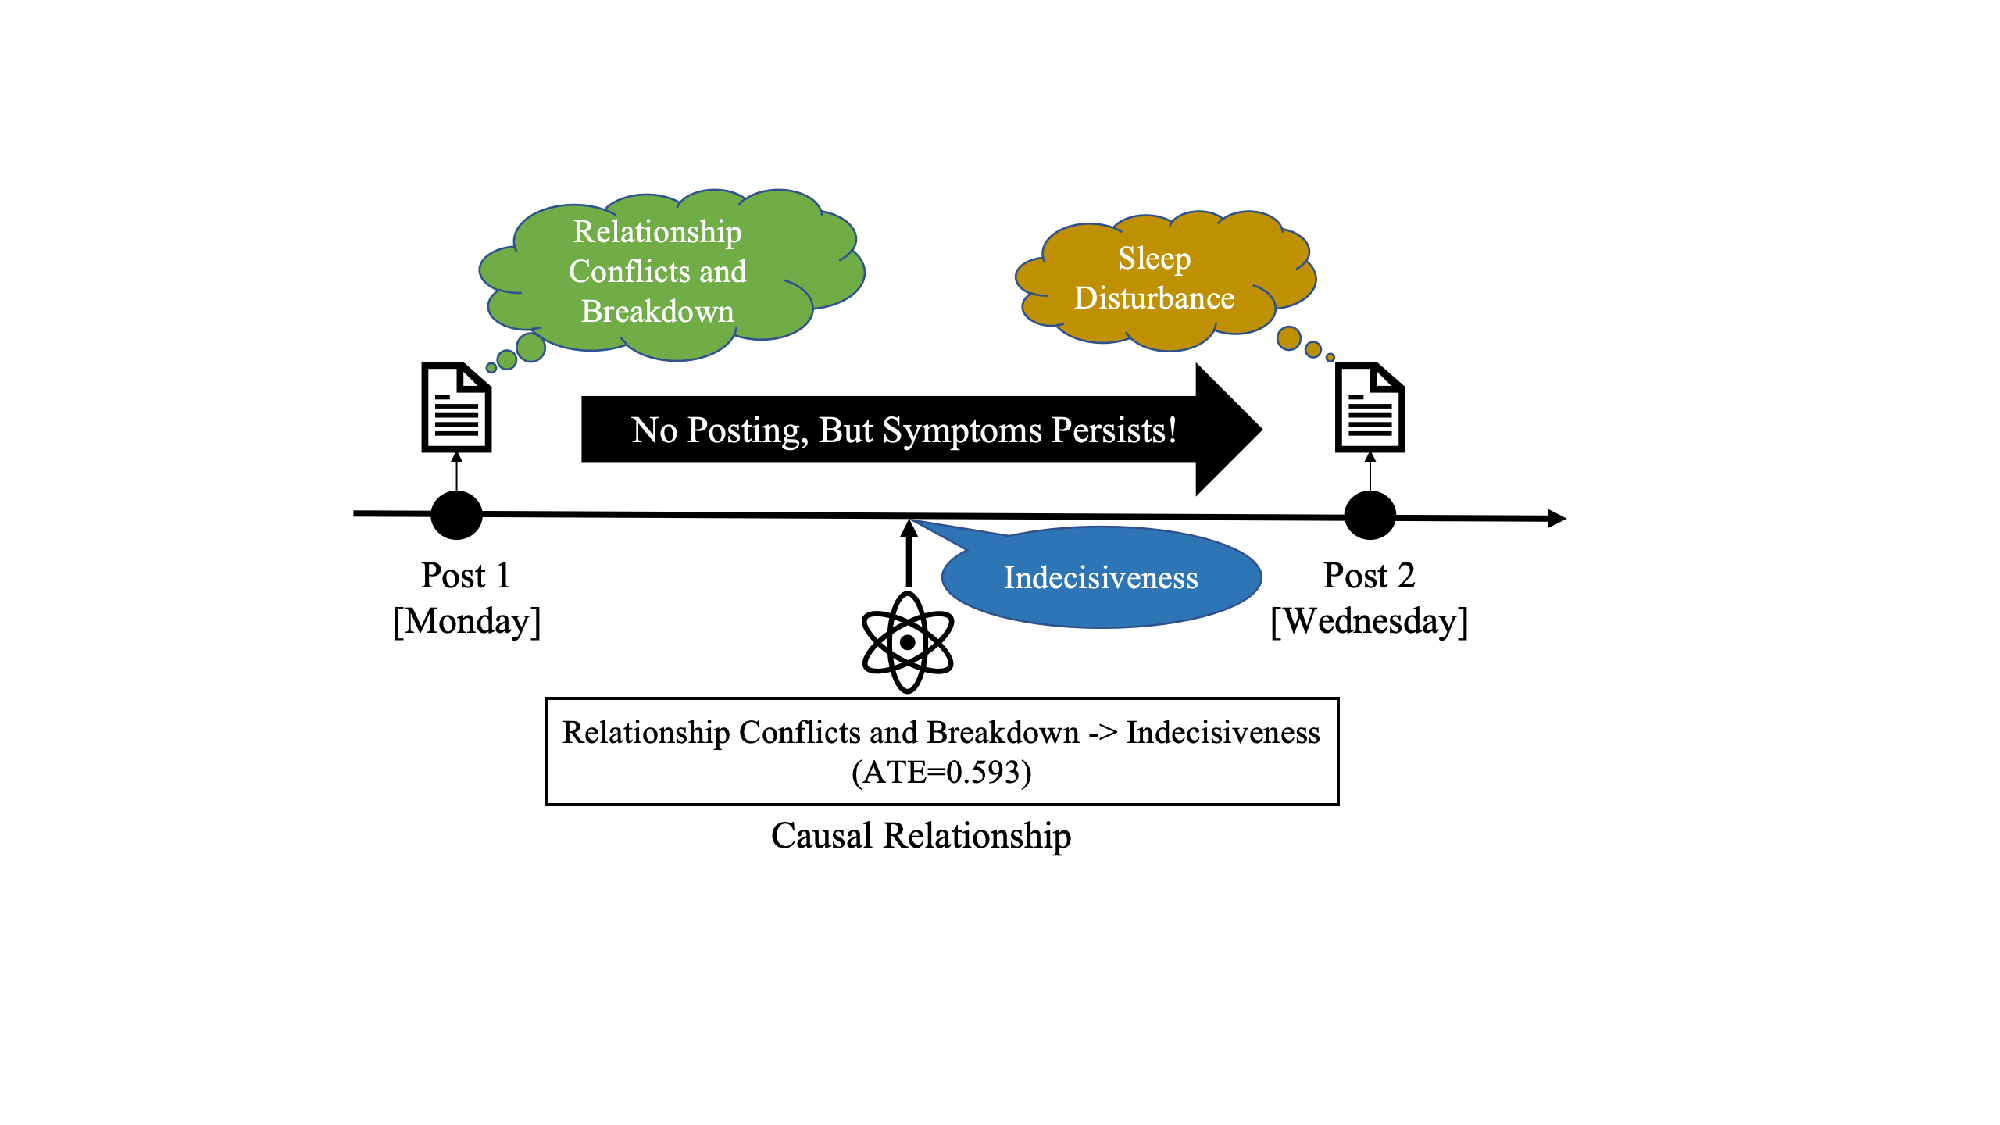
\includegraphics[width=\linewidth]{figures/causal_apply.pdf}
	\caption{Illustration of incomplete symptom sequence in social media posts, while causal relationships can help to replenish missing symptoms.}
	\label{fig:causal_apply}
\end{figure}



Let $S_D$ denote the original symptom vector of a user on day $D$. The adjusted symptom vector $S_D'$, considering the causal relationship, is calculated as follows:
\begin{equation}
    S_D'=S_D+ \frac{1}{W}C_{symp}^T\sum_{i=1}^W S_{D-i}
\end{equation}
Here, $C_{symp}$ represents the causal matrix, with $C_{symp}[i][j]$ indicating the Average Treatment Effect (ATE) of the $i$-th symptom causing the $j$-th symptom. The variable $W$ represents the time window. Therefore, the causal matrix can help us predict how much the probabilities of other symptoms will increase or decrease based on the symptom sequences $[S_{D-W}, ..., S_{D-1}]$ from the previous $W$ days, 

Similarly, we can adjust the original symptom vector using ``life-events-to-symptom'' causal relationship:
\begin{equation}
    S_D'=S_D+\frac{1}{W}C_{LE}^T\sum_{i=1}^W L_{D-i}
\end{equation}
Here, $C_{LE}$ represents the causal matrix, with $C_{LE}[i][j]$ indicating the ATE of the $i$-th life event causing the $j$-th symptom. $L_D$ denotes the life event vector on day $D$.



% Denoting the Causal matrix as $C_{symp}$, where $C_{symp}[i][j]$ represents the Average Treatment Effect (ATE) of the $i$-th symptom causing the $j$-th symptom. When symptom $s_t$ appears, the Causal matrix helps determine how much the probabilities of other symptoms increase or decrease.  $S_D$ refers to the symptom matrix of a user on day D, and $S_D'$ represents the user's symptom matrix after being adjusted by the causal matrix. We adjust the symptom matrix by applying the causal matrix to the average of the matrices from $D-30$ days and $D-1$ day and adding it to the original symptom matrix. 
% Similarly, the interpolation formula of ``life-events-to-symptom'' causal relationship is as follows:
% $$S_D'=S_D+C_{LE}^Tavg(L_{D-30},L_{D-1})$$


% Understanding the causality between symptoms allows us to identify whether the presence of symptom A makes it more likely for symptom B to occur or not. This property can be employed to adjust the probability vector of symptoms (38 dimensions) that changes over time. Let the Causal matrix (38 x 38) be denoted as $C_{symp}$, where $C_{symp}[i][j]$ represents the Average Treatment Effect (ATE) of the i-th symptom causing the j-th symptom. When symptom A appears, according to the Causal matrix, we can determine how much the probabilities of other symptoms increase or decrease. In both of these downstream task, we apply causality through interpolation. $S_D$ refers to the symptom matrix of a user on day D, and $S_D'$ represents the user's symptom matrix after being adjusted by the causal matrix. We adjust the symptom matrix by applying the causal matrix to the average of the matrices from $D-30$ days and $D-1$ day and adding it to the original symptom matrix. The interpolation formula is as follows:
% $$S_D'=S_D+C_{symp}^Tavg(S_{D-30},S_{D-1})$$
% Similarly, we applied the causality between life events and symptoms to the task of time point detection. The interpolation formula is as follows:
% $$S_D'=S_D+C_{LE}^Tavg(L_{D-30},L_{D-1})$$

% Additionally, we incorporate both causal results into two downstream tasks using the method outlined in the formula. $C_{symp}$ and $C_{LE}$ respectively denote the causal matrices between symptoms and between life events and symptoms. Similarly, we adjust the symptom matrix by applying the causal matrix to the average of the matrices from $D-30$ days and $D-1$ day, and the average of life events matrices, and then add it to the original symptom matrix to obtain the adjusted symptom matrix.
% \begin{equation*}
%     \begin{aligned}
% S_D'= S_D+C_{symp}^Tavg(S_{D-30},S_{D-1})
% \\+C_{LE}^Tavg(L_{D-30}, L_{D-1})
% \end{aligned}
% \end{equation*}



% Detecting the right moment for diagnosis is crucial as it can significantly impact the effectiveness of interventions, treatments, and overall prognosis.

% This can be a critical juncture for determining the appropriate interventions to address the condition and prevent it from worsening. Timely diagnosis can also lead to better management of symptoms and an improved quality of life for individuals affected by mental health issues. 

% siyuan: 感觉上面这一段翻来覆去都在讲一个意思“diagnosis point detection很有意义,能够使治疗、干预更及时”,需要变简洁一些。还需要在这里formalize一下这个任务的定义,然后在实验部分简要介绍写一下这个task的evaluation metric

%diagnosis point detection定义:
% Considering $p$ different users, for each user $i$($i\in\{1,...,p\}$), there are $n_i$ social media posts. The posts written by user $i$ are provided in chronological order: $P_1, ..., P_{n_i}$. Diagnosis Point Detection involves processing the post sequence of each user to determine the precise time point $l$($l\in {1,...,n_i}$) at which the user is diagnosed with a specific disease.
% We apply the causality obtained in the previous section to this work by interpolation.After we added the causality, the results of this work were improved, indicating that the causal effect we obtained before is effective. 
% siyuan:这一段有用的信息似乎只有“interpolation”,不需要在这里说加了casual之后效果提升了。建议直接把这一段去掉,然后在介绍完这两个任务之后,统一用一段讲一下我们怎么插值的



% \subsection{Task 2: Symptom Sequence Prediction}
% Symptom sequence prediction is a predictive modeling approach used in healthcare and medical research to forecast the likely progression of symptoms or clinical events over time. It involves analyzing historical data to identify patterns and relationships among symptoms, medical conditions, or events in order to predict the sequence in which they are likely to occur in the future. This approach is particularly valuable in various medical fields, including mental health, as it can provide insights into disease progression, treatment outcomes, and patient management.In the context of mental health, symptom sequence prediction aims to understand how different symptoms or manifestations of psychological disorders unfold over time. This can help clinicians and researchers anticipate the sequence of symptoms associated with a particular disorder, leading to more accurate diagnoses and tailored treatment strategies.
% Our task is to predict the symptoms that may appear in the next period given the sequence of symptoms that the user has experienced in the previous period.Given the previous sequence of symptoms, the model generates symptoms may appear in the next period of time.
% \subsection{Task 2: Early Detection of Depression}
% Previous research has demonstrated the benefits of early detection and treatment for depression, improving its negative impact and expediting the treatment process. Treating depression in its early stages is often more cost-effective than dealing with the consequences of untreated or poorly managed depression. Early intervention can prevent the need for more intensive and expensive treatments later on. For instance, \citet{halfin2007depression} has shown that early detection, intervention, and appropriate treatment can promote relief, prevent relapse, and reduce the emotional and economic burden of the illness. Early detection allows for immediate implementation of suitable interventions, including therapy, counseling, and, when necessary, medication. Initiating treatment in the early stages of depression is generally more effective and can prevent the worsening of the condition, as demonstrated by studies such as \citet{picardi2016randomised}, which highlight the significantly positive impact of early detection and treatment on the severity of depressive symptoms and the rate of improvement.

% Early detection of depression was proposed by \citet{losada2016test}, who integrated depression detection with the field of early detection and released the Reddit Early Detection Dataset. Considering $p$ different users, for each user $i$($i\in\{1,...,p\}$), there are $n_i$ social media posts. The posts written by user $i$ are provided in chronological order: $P_1, ..., P_{n_i}$. The task of early detection of depression involves processing each post sequence. At a specific point $k$($k\in\{1,...,n_i\}$), a binary decision must be made regarding whether user $i$ is a potential positive case for depression, aiming to detect positive cases as early as possible.
% siyuan: 这里只写了这个任务的重要性,没有把early detection的任务定义写清楚,也没有引用提出这个任务的原始的paper。同样的,把evaluation metric在实验部分写一下

% Social media posts may not necessarily fully reflect all symptoms of an individual. Therefore, we use causality to fill in incomplete symptom sequences. Subsequently, we apply the symptom sequences to these two downstream tasks.
